% ============================================================
% ALL FIGURES & TABLES — ordered by appearance in the paper
% Upload all files in this folder to your Overleaf project
% ============================================================

% --- Fig 1  (Section 4: Dataset) ---
\begin{figure}[t]
  \centering
  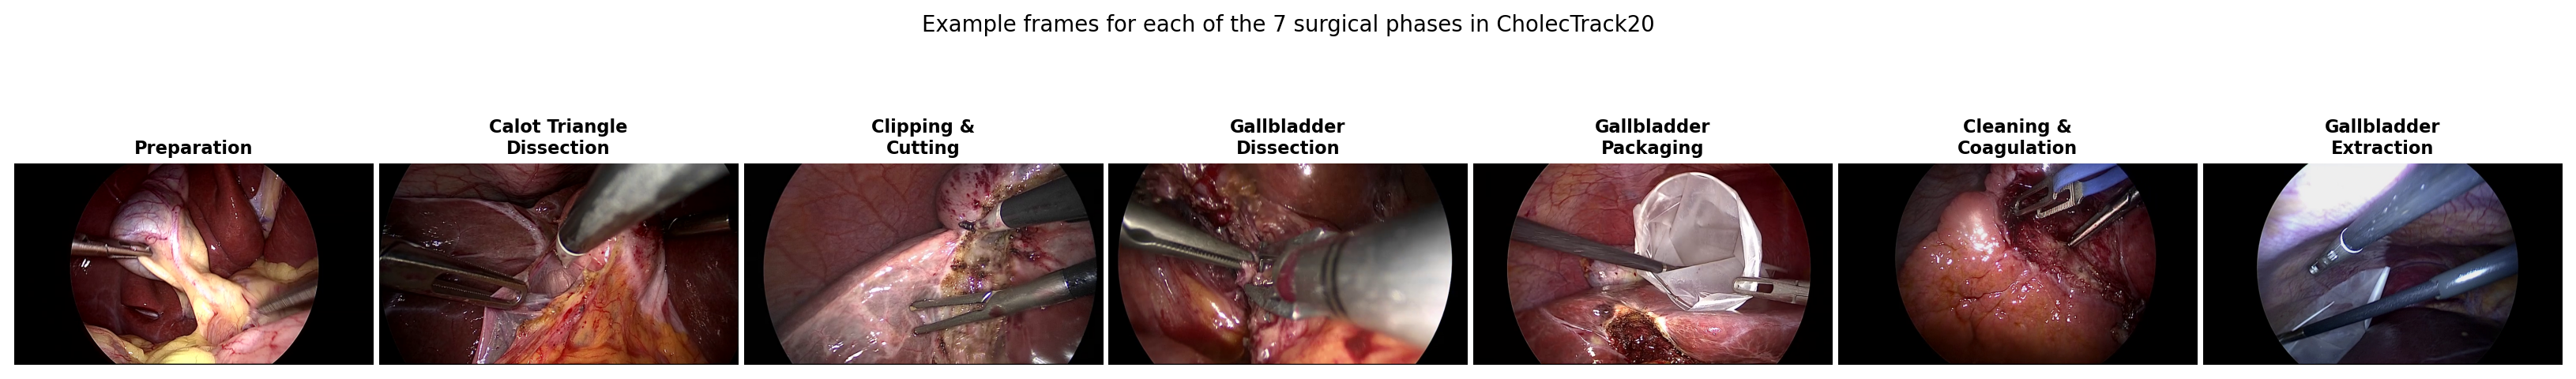
\includegraphics[width=\linewidth]{fig1_phase_examples.png}
  \caption{Representative 1-fps frames for each of the seven CholecTrack20 surgical phases. Calot Triangle Dissection and Gallbladder Dissection are visually similar, motivating macro-F1 as the primary metric.}
  \label{fig:phases}
\end{figure}

% --- Table (Section 4: Dataset) ---
\begin{table}[t]
  \centering
  \caption{Per-phase frame counts in the 12-video CholecTrack20 subset.}
  \label{tab:phases}
  \begin{tabular}{lcc}
  \toprule
  Phase & Frames & \% of total \\
  \midrule
  CalotTriangleDissection & 10,289 & 53.1\% \\
  ClippingCutting & 4,785 & 24.7\% \\
  GallbladderDissection & 1,388 & 7.2\% \\
  CleaningCoagulation & 1,166 & 6.0\% \\
  Preparation & 815 & 4.2\% \\
  GallbladderPackaging & 536 & 2.8\% \\
  GallbladderExtraction & 411 & 2.1\% \\
  \midrule
  Total & 19,390 & 100\% \\
  \bottomrule
  \end{tabular}
\end{table}

% --- Fig 2  (Section 5: Frozen results) ---
\begin{figure}[t]
  \centering
  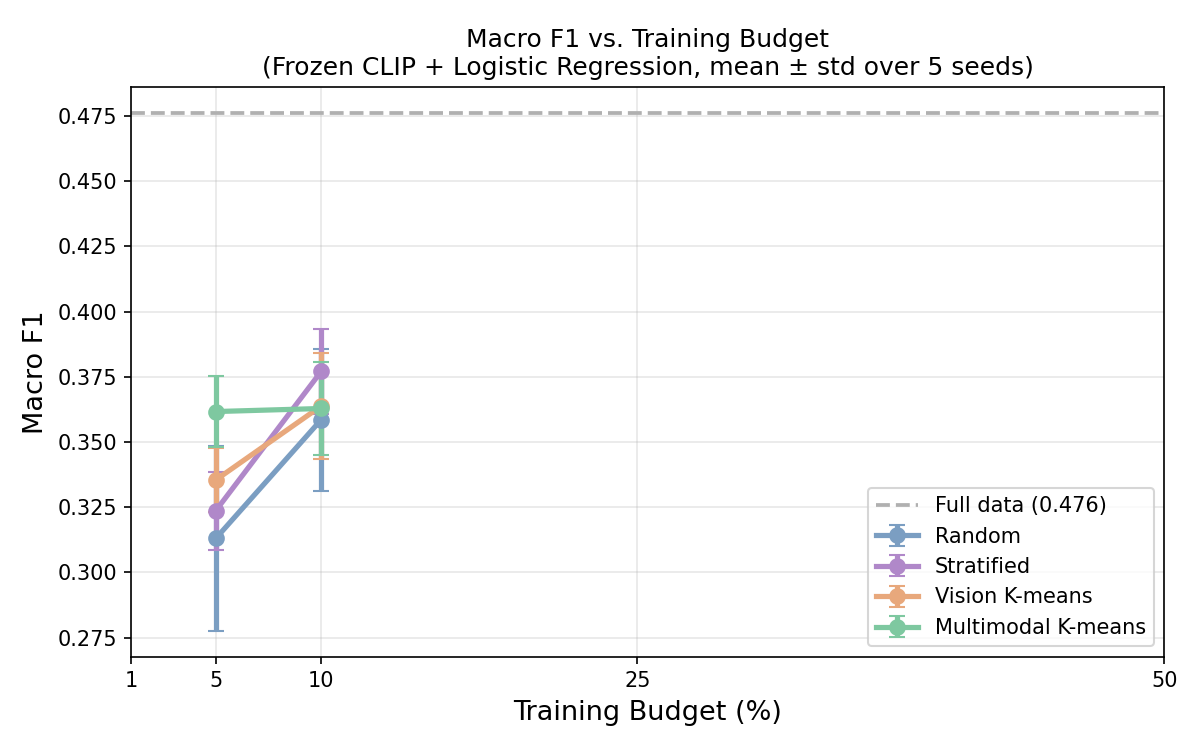
\includegraphics[width=\linewidth]{fig2_perf_vs_budget.png}
  \caption{Macro-F1 vs.\ training-data budget for all four samplers (mean $\pm$ std over 5 seeds). The dashed line is the full-data upper bound. Multimodal K-means leads at the 5\% budget; methods converge at 10\% and above.}
  \label{fig:perf_vs_budget}
\end{figure}

% --- Table X  (Section 5: Frozen results) ---
\begin{table}[t]
  \centering
  \caption{Frozen-feature macro-F1 (mean $\pm$ std, 5 seeds) at the 5\% and 10\% budgets.}
  \label{tab:frozen}
  \begin{tabular}{lcc}
  \toprule
  Method & 5\% Budget & 10\% Budget \\
  \midrule
  Random & 0.313 $\pm$ 0.035 & 0.359 $\pm$ 0.027 \\
  Stratified & 0.324 $\pm$ 0.015 & 0.377 $\pm$ 0.016 \\
  Vision K-means & 0.335 $\pm$ 0.012 & 0.364 $\pm$ 0.020 \\
  \textbf{Multimodal K-means} & \textbf{0.362 $\pm$ 0.013} & 0.363 $\pm$ 0.018 \\
  \midrule
  Full data (100\%) & --- & 0.476 \\
  \bottomrule
  \end{tabular}
\end{table}

% --- Fig 3  (Section 5: Fine-tuning results) ---
\begin{figure}[t]
  \centering
  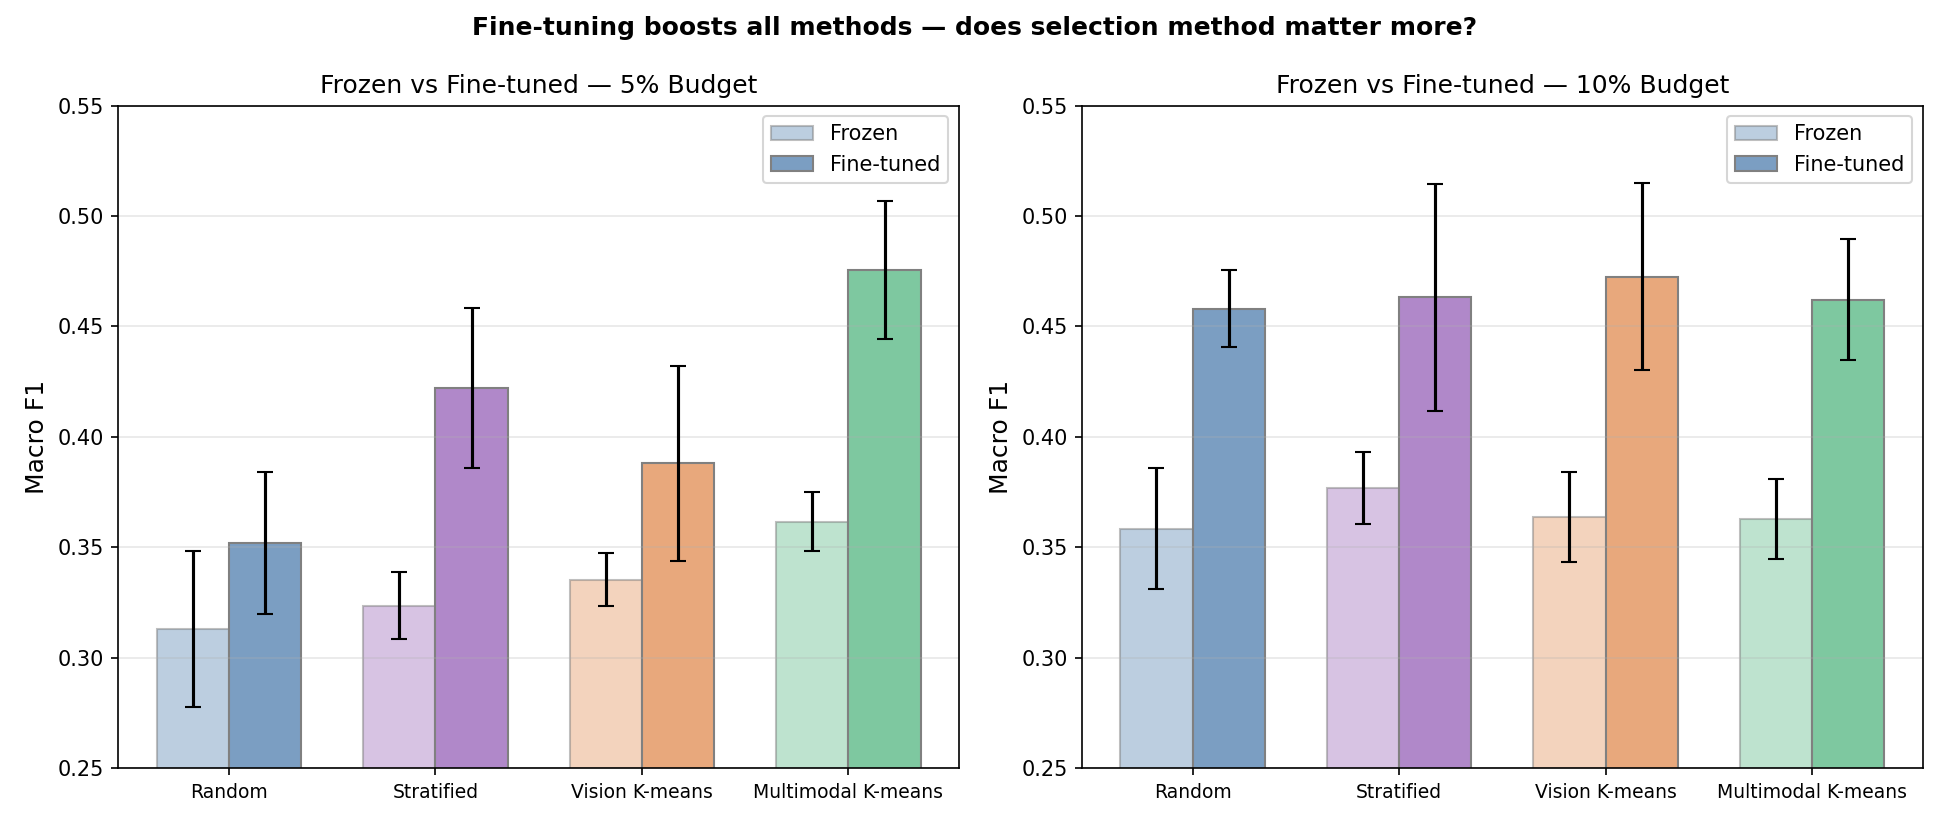
\includegraphics[width=\linewidth]{fig3_frozen_vs_finetuned.png}
  \caption{Macro-F1 of frozen (light) vs.\ fine-tuned (solid) classifiers at the 5\% and 10\% budgets. Fine-tuning amplifies all methods; multimodal selection gains most at the 5\% budget.}
  \label{fig:frozen_vs_ft}
\end{figure}

% --- Table Y  (Section 5: Fine-tuning results) ---
\begin{table}[t]
  \centering
  \caption{Fine-tuned macro-F1 (mean $\pm$ std, 2 seeds) at the 5\% and 10\% budgets.}
  \label{tab:finetuned}
  \begin{tabular}{lcc}
  \toprule
  Method & 5\% Budget & 10\% Budget \\
  \midrule
  Random & 0.352 $\pm$ 0.032 & 0.458 $\pm$ 0.017 \\
  Stratified & 0.422 $\pm$ 0.036 & 0.463 $\pm$ 0.051 \\
  Vision K-means & 0.388 $\pm$ 0.044 & 0.473 $\pm$ 0.042 \\
  \textbf{Multimodal K-means} & \textbf{0.476 $\pm$ 0.031} & 0.462 $\pm$ 0.028 \\
  \bottomrule
  \end{tabular}
\end{table}

% --- Fig 4  (Section 5: Qualitative analysis) ---
\begin{figure}[t]
  \centering
  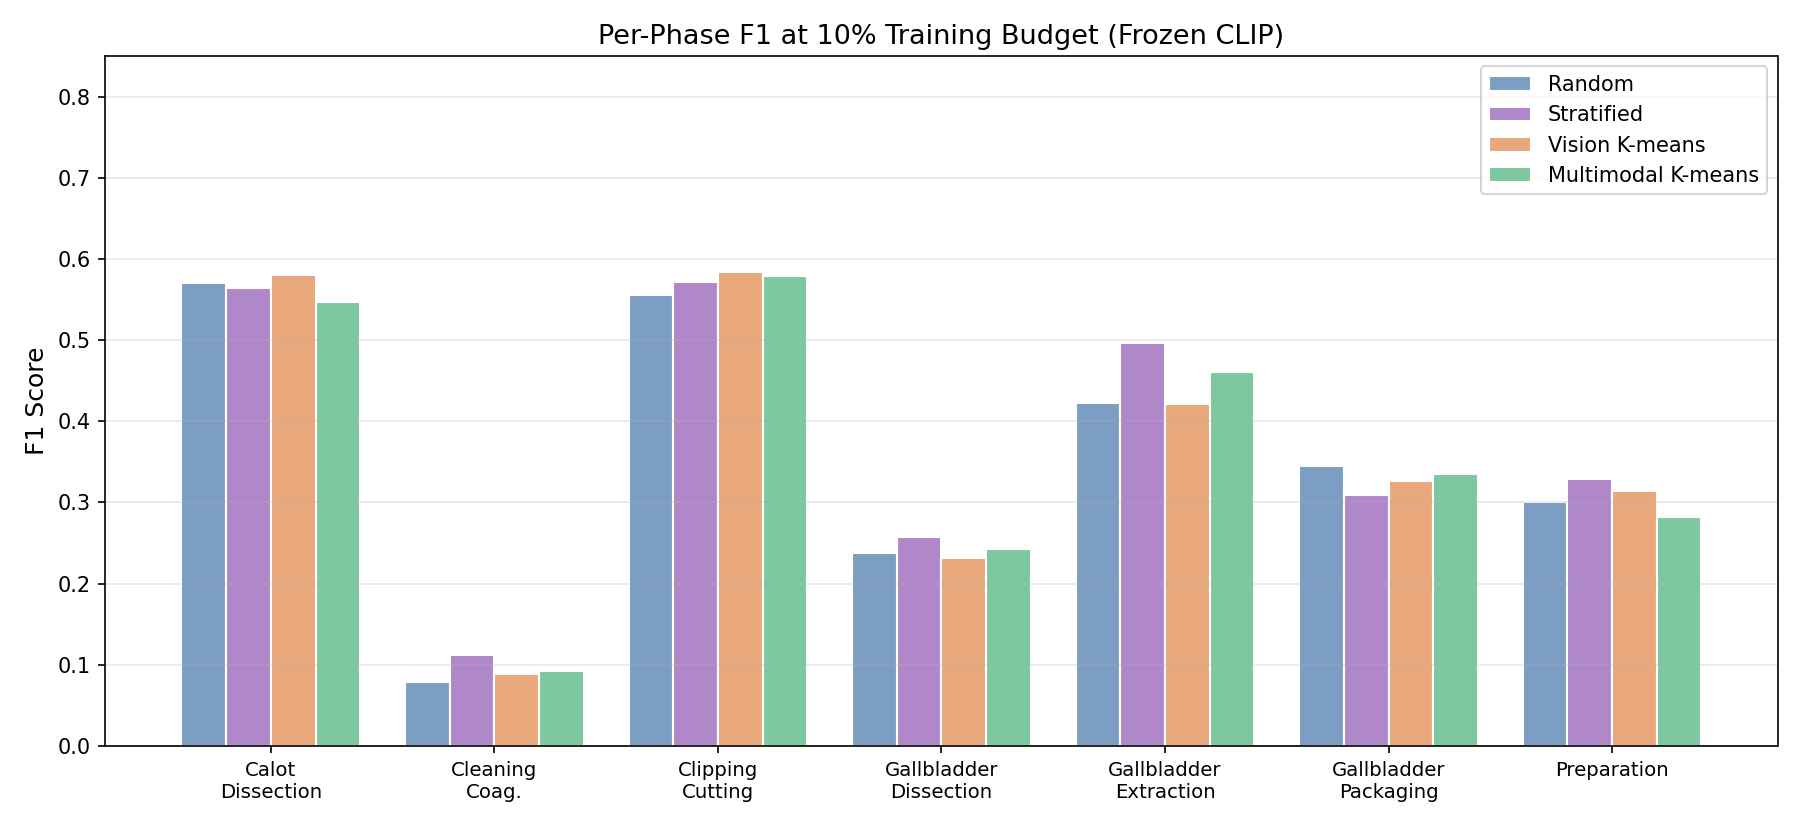
\includegraphics[width=\linewidth]{fig4_per_class_f1.png}
  \caption{Per-phase F1 at the 10\% training budget (frozen CLIP). CleaningCoagulation and GallbladderDissection are consistently the hardest phases across all sampling methods.}
  \label{fig:perclass}
\end{figure}

% --- Fig 5  (Section 5: Qualitative analysis) ---
\begin{figure}[t]
  \centering
  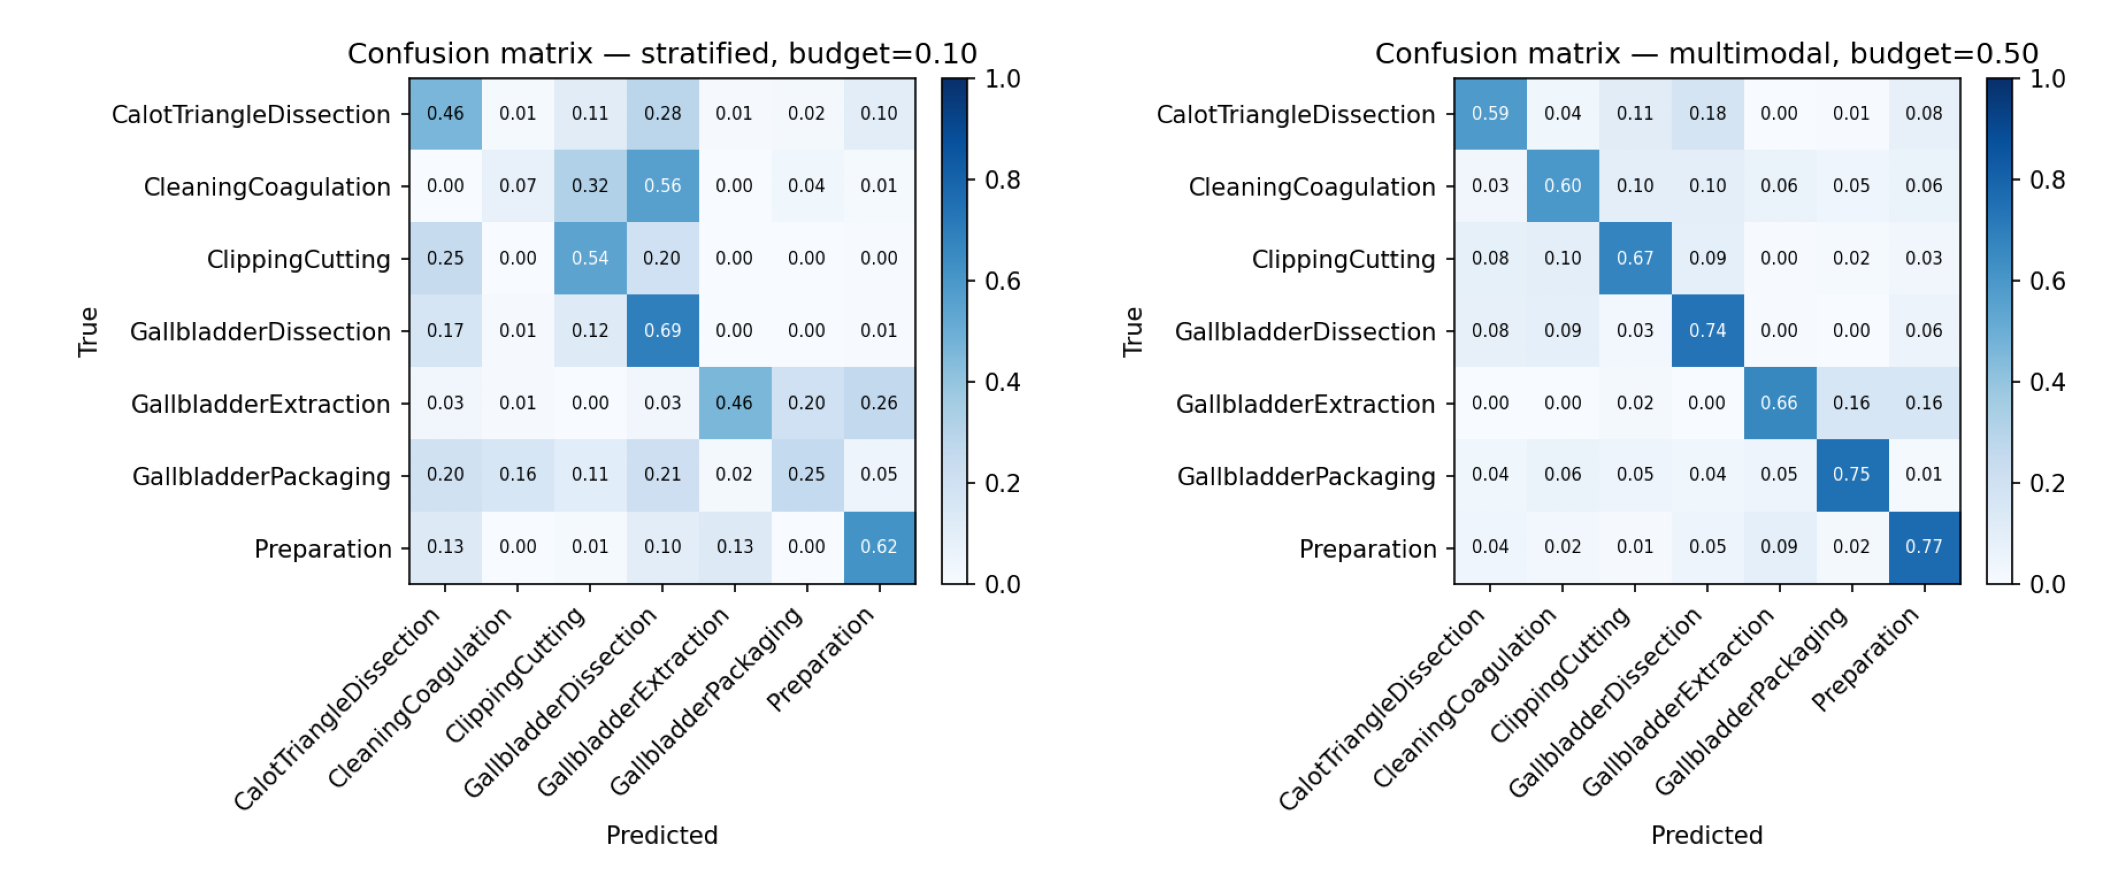
\includegraphics[width=\linewidth]{fig5_confusion_matrices.png}
  \caption{Confusion matrices for the stratified sampler at 10\% budget (left) and multimodal K-means at 50\% budget (right). GallbladderDissection is systematically confused with CalotTriangleDissection due to visual similarity.}
  \label{fig:cm}
\end{figure}
